\section{Grafteori}

Grafteori handler om at beskrive  modeller matematisk. Grafteori er væslig når man skal optimere et netværk, og derfor bruges det bla inden for rutefinding, hvor grafen kunne f.eks. representere et vejnetværk. 
En graf beskriver et par af mægnder, man kunne tag udgangspunkt i grafen G = (V,E) hvor V og E er mægnder. I eksempet her er V en ikke-tom mængde af knuder, og E er mængden af kanter som forbinder knuderne i mægnden V (En kant kan godt forbinde den samme knude, dette kaldes en løkke). 

\vspace{5mm}

Vi tager udgangpunkt i grafen.

\begin{figure}[H]
\begin{adjustbox}{width=1.2\textwidth,center=\textwidth}
\centering
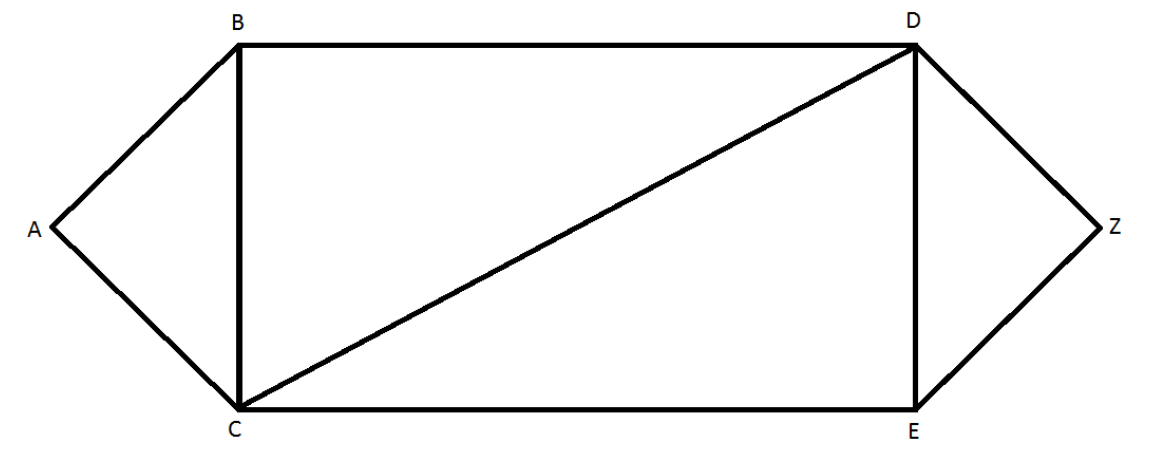
\includegraphics[width=1.2\textwidth]{Pictures/Teoriafsnit/Figurfiler/Grafteori_graf.png}
\end{adjustbox}
\caption{Et simpel vejnetværk}
\label{fig:grafteori}
\end{figure}

Man kan forstille sig dette er et vejnetværk, hvor punkterne(knuderne) representere byer, og linjerne(kanterne) er veje som forbinder byerne.

\vspace{5mm}

Vi kan udfra grafen se at knuderne \verb"A, B, C, D, E, Z \in V"!. Samt at kanterne \verb!"{A,B} , {A,C} , {B,C} , {B,D} , {C,E} , {C,D} , {D,E} , {D,Z} , {E,Z} \in E"!

\vspace{5mm}

Grafen her kan derfor skrives rent matematisk:

\vspace{5mm}

\verb!G = (V,E) og V = {A,B,C,D,E,Z} og E = { {A,B} , {A,C} , {B,C} , {B,D} , {C,E} , {C,D} , {D,E} , {D,Z} , {E,Z} }!

\vspace{5mm}

En anden måde at repræsentere grafen på er ved hjælp af en adjacency matrix VxE, hvor v1, v2...vn, er knuderne, og e1, e2...en, er kanterne. I matrixen beskrives forbindelser mellem 2 knuder med 1 taller, hvor 0 beskriver ingen forbindelse mellem de 2 knuder.


\begin{figure}[H]
\begin{adjustbox}{width=1.2\textwidth,center=\textwidth}
\centering
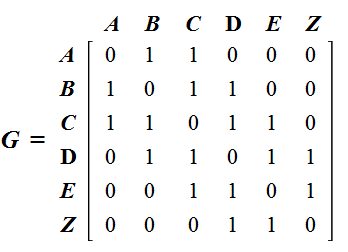
\includegraphics[width=1.2\textwidth]{Pictures/Teoriafsnit/Figurfiler/Grafteori_matrix.png}
\end{adjustbox}
\caption{Adjacency matrix}
\label{fig:grafteori}
\end{figure}


Grafteori er derfor et vigtigt emne, da f.eks. korteste rute algoritmer som Dijkstra's har brug for at vide hvordan knuderne er forbundet, samt graden(hvor mange kanter knuden har) af den enktle knude, for at kun udregne den korteste rute. Derudover vil grafmetoder som nabo-matrixen være en god måde at beskrive en grafs mægnder i programerings niveau. 